\subsection{\href{http://www.digicard.com.ar/}{Digicard S.A.}}
   \hypertarget{subsec:digicard}
   Durante varios anos se trabajo para la empresa en el area de desarrollo de nuevos productos de hardware orientados al control de accesos. Se puede destacar el desarrollo de un nuevo lector RFID de 125khz para reemplazar los lectores importados y a su vez proveer soluciones customizadas e integradas con el resto del sistema de control de accesos de la empresa. Se realizo la toma de requerimientos, el diseño esquematico, PCB, prototipo, documentación para producción y puesta en marcha, y documentación de uso. El lector se continua produciendo y utilizando actualmente  Algunas fotos del equipo se pueden ver en la figura \ref{fig:digicard}.
   \begin{figure}
      \begin{center}
         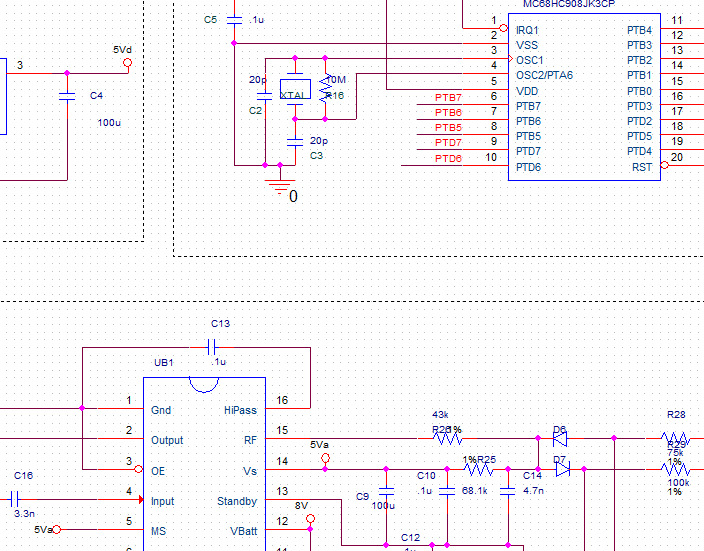
\includegraphics[width=0.24\textwidth]{digicard1.jpg}
         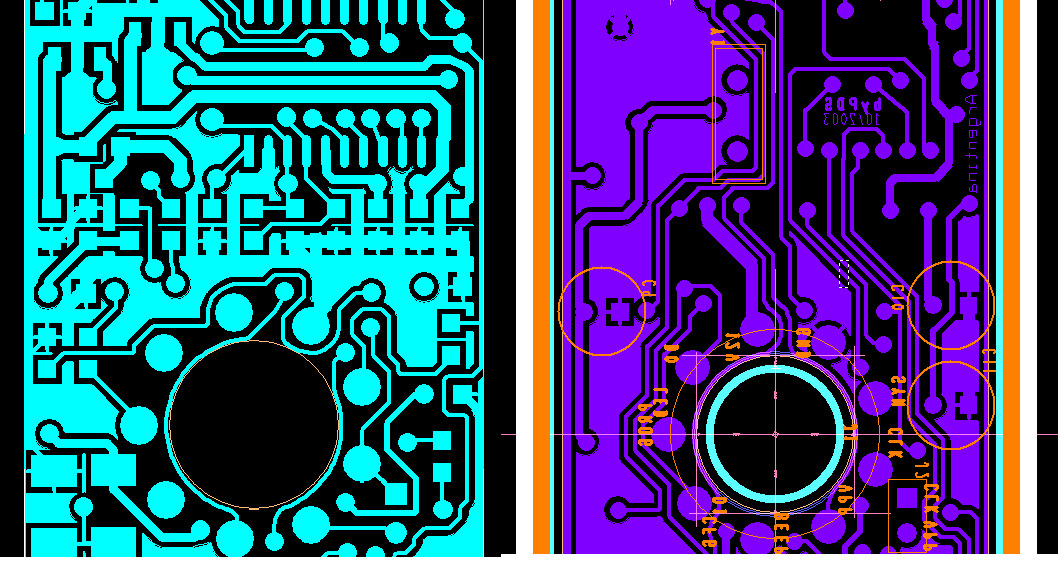
\includegraphics[width=0.24\textwidth]{digicard2.jpg}
         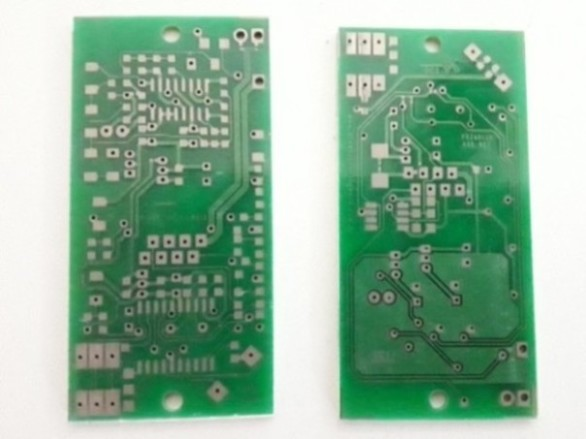
\includegraphics[width=0.24\textwidth]{digicard3.jpg}
         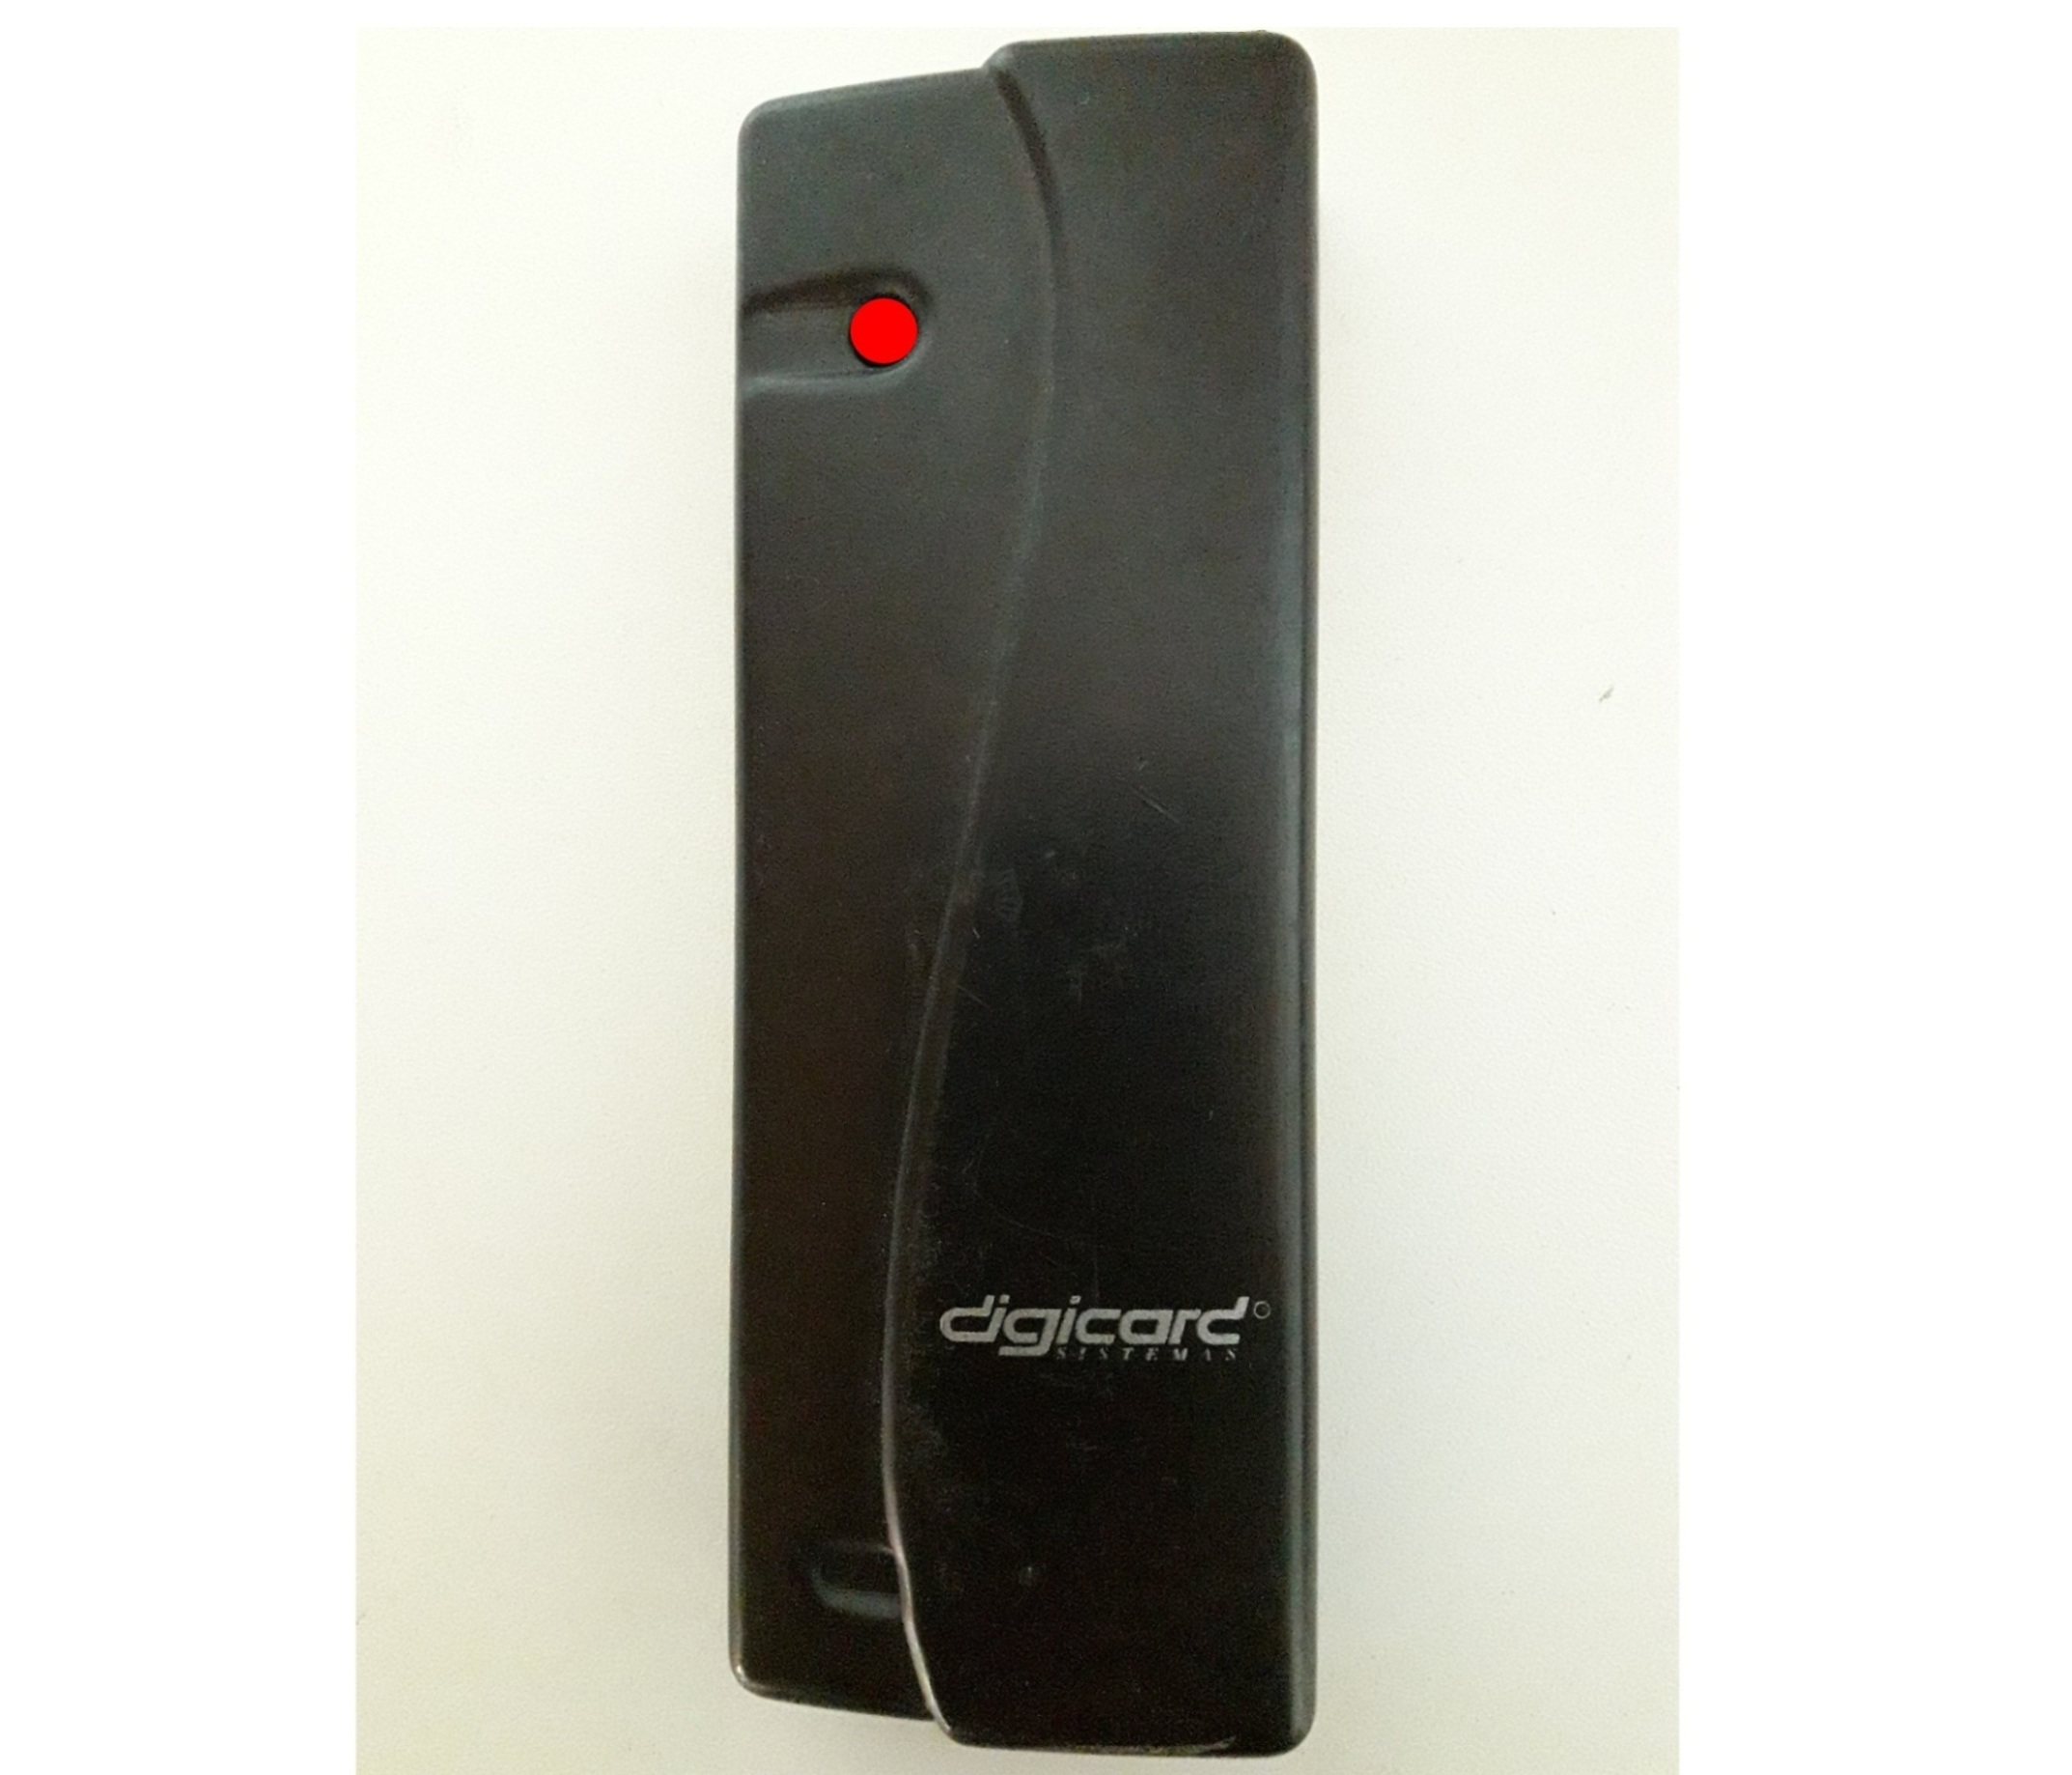
\includegraphics[width=0.24\textwidth]{digicard4.jpg}
      \end{center}
      \caption{Desarrollo de hardware, firmware y producción de lector de RFID de 125khz para la empresa Digicard.}
      \label{fig:digicard}
   \end{figure}
